\graphicspath{ {./first_steps/pictures/} }
\section{First steps}
\subsection{Get Started}
\begin{enumerate}
\item Connect the USB-to-TTL module together with the ESP32S-CAM board  to one free USB-Port on your pc. The setup of the board-connections, can you see in picture~\ref{ESP32-CAM-USB-TO-TTL}.
\item Check which port has this USB-to-TTL module get from your OS. You can check this with \texttt{ls -lisa /dev/ttyUSB*} (here in our example it is \texttt{/dev/ttyUSB0}).
\item Run in a terminal \texttt{get\_idf}, what we have introduce in section~\nameref{environment_variable}.
\item Create in a terminal the folder-structure, where you want to add the hello\_world-example. Here we put the hello\_world-example under \texttt{~/esp}:
\begin{lstlisting}[language=bash]
$ mkdir ~/esp
$ cd ~/esp
$ cp -r $IDF_PATH/examples/get-started/hello_world . 
\end{lstlisting} 
\item Now to compile the hello\_world-sources, run \texttt{idf.py build}
\begin{lstlisting}[language=bash]
$ idf.py build
Executing action: all (aliases: build)
...
-- Configuring done
-- Generating done
...
build/bootloader
[874/884] Performing build step for 'bootloader'
[1/3] Linking C executable bootloader.elf
[2/3] Generating binary image from built executable
esptool.py v3.3-dev
Creating esp32 image...
Merged 1 ELF section
Successfully created esp32 image.
...
or run 'idf.py -p (PORT) flash'
$
\end{lstlisting}
\item Run as last step the flash-command:
\begin{lstlisting}[language=bash]
$ idf.py -p /dev/ttyUSB0 flash 
Executing action: flash
...
hello_world.bin binary size 0x29840 bytes. Smallest app partition is 0x100000 bytes. 0xd67c0 bytes (84%) free.
[2/5] Performing build step for 'bootloader'
...
esptool.py v3.3-dev
Serial port /dev/ttyUSB0
Connecting....
Chip is ESP32-D0WDQ6 (revision 1)
Features: WiFi, BT, Dual Core, 240MHz, VRef calibration in efuse, Coding Scheme None
Crystal is 40MHz
MAC: 78:21:84:7d:01:78
Uploading stub...
Running stub...
Stub running...
Changing baud rate to 460800
Changed.
Configuring flash size...
Flash will be erased from 0x00001000 to 0x00007fff...
Flash will be erased from 0x00010000 to 0x00039fff...
Flash will be erased from 0x00008000 to 0x00008fff...
Compressed 25424 bytes to 15904...
Writing at 0x00001000... (100 %)
Wrote 25424 bytes (15904 compressed) at 0x00001000 in 0.8 seconds (effective 240.1 kbit/s)...
Hash of data verified.
Compressed 170048 bytes to 89645...
Writing at 0x00010000... (16 %)
Writing at 0x0001b0ec... (33 %)
Writing at 0x0002087d... (50 %)
Writing at 0x00026035... (66 %)
Writing at 0x0002e652... (83 %)
Writing at 0x00036a4a... (100 %)
Wrote 170048 bytes (89645 compressed) at 0x00010000 in 2.5 seconds (effective 552.7 kbit/s)...
Hash of data verified.
Compressed 3072 bytes to 103...
Writing at 0x00008000... (100 %)
Wrote 3072 bytes (103 compressed) at 0x00008000 in 0.1 seconds (effective 307.1 kbit/s)...
Hash of data verified.

Leaving...
Hard resetting via RTS pin...
Done
$
\end{lstlisting}
\item If you got the following,
\begin{lstlisting}
$ idf.py -p /dev/ttyUSB0 flash
Executing action: flash
...
esptool.py v3.3-dev
Serial port /dev/ttyUSB0
Connecting..................
...
$
\end{lstlisting}
you have to press the reset-button (see here \ref{ESP32-S-CAM-reset-button} or here \ref{ESP32-CAM-backside}), that the board goes into
the flash-mode. Then it starts to flash the ESP32S-CAM Board \cite{EspressifGetStartedGetESPIDF}.

\begin{figure}[H]
\centering
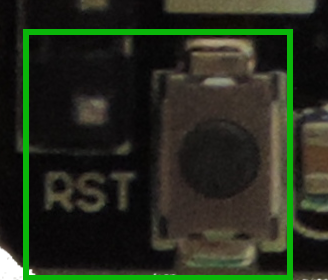
\includegraphics[width=0.25\textwidth]{reset_button}
\caption[ESP32-S-CAM Reset Button]{ESP32-S CAM Reset Button \\ Source: own picture}
\label{ESP32-S-CAM-reset-button}
\end{figure}

\end{enumerate}

\subsection{Test of Hello World Example}
\begin{enumerate}
\item Disconnect the USB-Cable from the USB-to-TTL-Board and the pc, that the boards are currentless. 
\item Remove the cable between GND and IO0.
\item Connect again the USB-Cable to the USB-to-TTL-Board.
\item Now open again a terminal and run \texttt{get\_idf}.
\item Our Example is printing Hello World on terminal over a serial connection. Below you will see the command to open the serial port and also the successful output:
\begin{lstlisting}
$ idf.py -p /dev/ttyUSB0 monitor
--- idf_monitor on /dev/ttyUSB0 115200 ---
--- Quit: Ctrl+] | Menu: Ctrl+T | Help: Ctrl+T followed by Ctrl+H ---
Restarting in 3 seconds...
Restarting in 2 seconds...
Restarting in 1 seconds...
Restarting in 0 seconds...
Restarting now.
ets Jun  8 2016 00:22:57

rst:0xc (SW_CPU_RESET),boot:0x13 (SPI_FAST_FLASH_BOOT)
configsip: 0, SPIWP:0xee
clk_drv:0x00,q_drv:0x00,d_drv:0x00,cs0_drv:0x00,hd_drv:0x00,wp_drv:0x00
mode:DIO, clock div:2
load:0x3fff0030,len:6752
load:0x40078000,len:14796
load:0x40080400,len:3792
0x40080400: _init at ??:?

entry 0x40080694
I (27) boot: ESP-IDF v5.0-dev-1452-g93106c9348 2nd stage bootloader
I (27) boot: compile time 16:08:09
I (27) boot: chip revision: 1
I (31) boot_comm: chip revision: 1, min. bootloader chip revision: 0
I (39) boot.esp32: SPI Speed      : 40MHz
I (43) boot.esp32: SPI Mode       : DIO
I (48) boot.esp32: SPI Flash Size : 2MB
I (52) boot: Enabling RNG early entropy source...
I (58) boot: Partition Table:
I (61) boot: ## Label            Usage          Type ST Offset   Length
I (69) boot:  0 nvs              WiFi data        01 02 00009000 00006000
I (76) boot:  1 phy_init         RF data          01 01 0000f000 00001000
I (83) boot:  2 factory          factory app      00 00 00010000 00100000
I (91) boot: End of partition table
I (95) boot_comm: chip revision: 1, min. application chip revision: 0
I (102) esp_image: segment 0: paddr=00010020 vaddr=3f400020 size=0782ch ( 30764) map
I (122) esp_image: segment 1: paddr=00017854 vaddr=3ffb0000 size=0243ch (  9276) load
I (126) esp_image: segment 2: paddr=00019c98 vaddr=40080000 size=06380h ( 25472) load
I (140) esp_image: segment 3: paddr=00020020 vaddr=400d0020 size=14978h ( 84344) map
I (171) esp_image: segment 4: paddr=000349a0 vaddr=40086380 size=04e64h ( 20068) load
I (180) esp_image: segment 5: paddr=0003980c vaddr=50000000 size=00010h (    16) load
I (186) boot: Loaded app from partition at offset 0x10000
I (186) boot: Disabling RNG early entropy source...
I (202) cpu_start: Pro cpu up.
I (202) cpu_start: Starting app cpu, entry point is 0x40081004
0x40081004: call_start_cpu1 at cpu_start.c:152

I (189) cpu_start: App cpu up.
I (217) cpu_start: Pro cpu start user code
I (217) cpu_start: cpu freq: 160000000 Hz
I (217) cpu_start: Application information:
I (221) cpu_start: Project name:     hello_world
I (227) cpu_start: App version:      1
I (231) cpu_start: Compile time:     Feb 11 2022 17:57:03
I (237) cpu_start: ELF file SHA256:  273a35a73851882c...
I (243) cpu_start: ESP-IDF:          v5.0-dev-1452-g93106c9348
I (250) heap_init: Initializing. RAM available for dynamic allocation:
I (257) heap_init: At 3FFAE6E0 len 00001920 (6 KiB): DRAM
I (263) heap_init: At 3FFB2D30 len 0002D2D0 (180 KiB): DRAM
I (269) heap_init: At 3FFE0440 len 00003AE0 (14 KiB): D/IRAM
I (276) heap_init: At 3FFE4350 len 0001BCB0 (111 KiB): D/IRAM
I (282) heap_init: At 4008B1E4 len 00014E1C (83 KiB): IRAM
I (289) spi_flash: detected chip: generic
I (293) spi_flash: flash io: dio
W (297) spi_flash: Detected size(4096k) larger than the size in the binary image header(2048k). Using the size in the binary image header.
I (311) cpu_start: Starting scheduler on PRO CPU.
I (0) cpu_start: Starting scheduler on APP CPU.
Hello world!
This is esp32 chip with 2 CPU core(s), WiFi/BT/BLE, silicon revision 1, 2MB external flash
Minimum free heap size: 296120 bytes
...
\end{lstlisting}
\end{enumerate}